\documentclass[a4paper]{article}
\usepackage[top=0.5cm, bottom=0cm, left=0.5cm, right=0.5cm]{geometry}
\usepackage{tikz}
\usetikzlibrary{patterns}
\usetikzlibrary{shapes,arrows}
\usetikzlibrary{decorations.pathreplacing, positioning}

\begin{document}
\noindent
  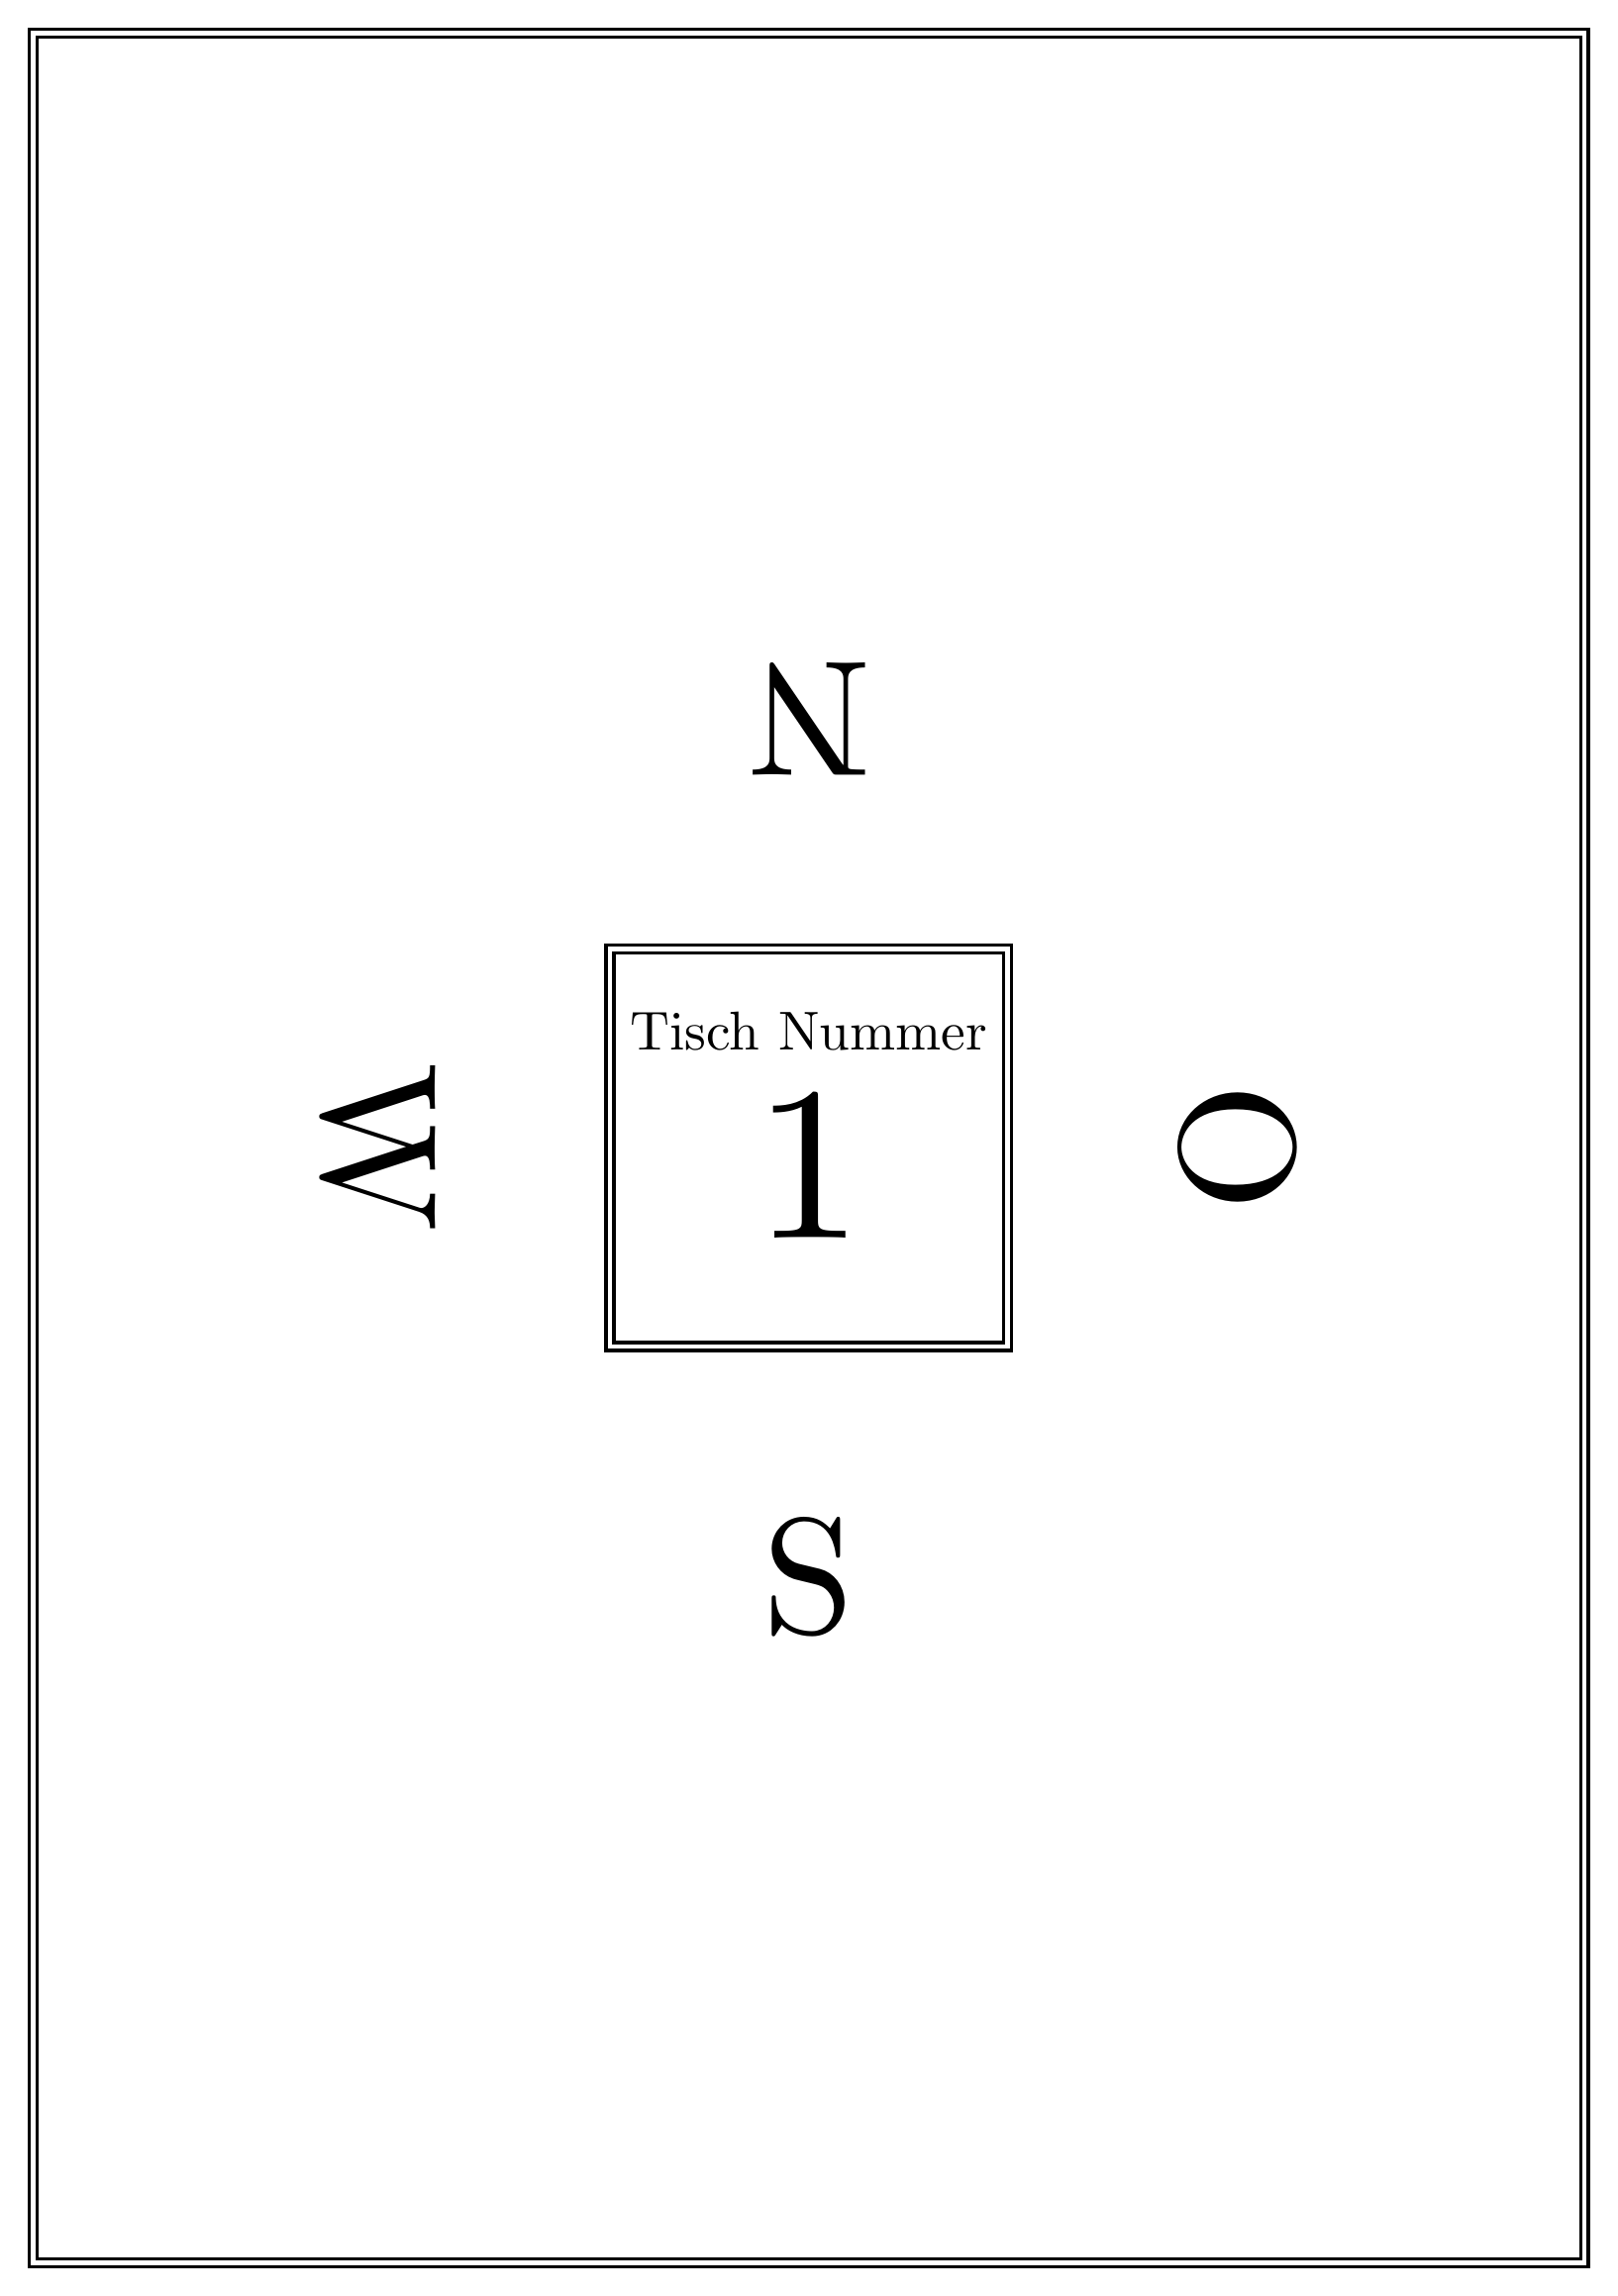
\begin{tikzpicture}

    % Border
    \draw[very thick] (0cm,0cm) rectangle (20.cm,28.7cm);
    \draw[very thick] (0.1cm,0.1cm) rectangle (19.9cm,28.6cm);

    % Table Nr
    \draw[very thick] (7.4cm,11.75) rectangle (12.6cm,16.95cm);
    \draw[very thick] (7.5cm,11.85) rectangle (12.5cm,16.85cm);

    \node[very thick, scale=2] at (10cm, 15.85cm) {Tisch Nummer};
    \node[very thick, scale=8] at (10cm, 14.1cm) {1};


    % Player Direction
    \node[very thick, scale = 6] at (10cm, 8.85cm) {S};

    \node[very thick, scale = 6, rotate=180] at (10cm, 19.85cm) {N};

    \node[very thick, scale = 6, rotate=270] at (4.5cm, 14.35cm) {W};

    \node[very thick, scale = 6, rotate=90] at (15.5cm, 14.35cm) {O};


    \end{tikzpicture}%
\end{document}
